\documentclass{beamer}    
% Theme
\usetheme{Madrid}
\usepackage{hyperref}
\hypersetup{
	colorlinks=false,
	linkcolor=blue,
	filecolor=blue,      
	urlcolor=blue,
}
\usepackage{pdfpages}
\usepackage{graphicx}
\usepackage{natbib}
\usepackage{lipsum}
\usepackage{arydshln}
\def\boxit#1{%
	\smash{\color{red}\fboxrule=1pt\relax\fboxsep=2pt\relax%
		\llap{\rlap{\fbox{\vphantom{0}\makebox[#1]{}}}~}}\ignorespaces
}
\renewcommand{\today}{\ifcase \month \or January\or February\or March\or %
	April\or May \or June\or July\or August\or September\or October\or November\or %
	December\fi, \number \year} 




% \AtBeginSection[]
% {
% 	\begin{frame}{Table of Contents}
% 		% \scriptsize
% 			\tableofcontents[hideallsubsections,hideothersubsections,currentsection]
% 	\end{frame}
% }	

% Title page
\title[Rationalising with agents’ heterogeneity]{ \textbf{Rationalising with agents’ heterogeneity}}
\subtitle{based on\\ \textit{\cite{aguiar2023hand}} and \textit{\cite{kaplan2014model}}}
\author[Morteza]{Seyyed Morteza Aghajanzadeh}
\institute[HH Finance]{Households Finance}
\date{\today}

\begin{document}

\begin{frame}
    \titlepage
\end{frame}

\begin{frame}
	\frametitle{Table of Contents}
	\tableofcontents[hideallsubsections]
\end{frame}

\section{Introduction}
\begin{frame}{Introduction}
	\begin{itemize}
		\item<1-> \textbf{Marginal Propensity to Consume (MPC)}:
		\begin{itemize}
			\item The increase in personal consumer spending (consumption) occurs with an increase in disposable income:
			\begin{equation*}
				MPC = \frac{\Delta C}{\Delta Y}
			\end{equation*}
		\end{itemize}
		\item<2-> We overviewed the Measurement of the MPC.
	\end{itemize}
\end{frame}

\begin{frame}{Introduction}
	\begin{itemize}
		\item<1-> Off-the-shelf models of consumption predict that the MPC should be negligible in the aggregate. 
		\begin{itemize}
			\item \cite{heathcote2009quantitative} provide a good survey of these models.
		\end{itemize}
		\item<2-> However, the empirical literature has found that the MPC is large and varies substantially across households.
		\begin{itemize}
			\item Collective evidence suggests that the MPC is around \textbf{0.25}.
			\item Higher MPC for lower wealth or liquidity households.
			\item Let's call this characteristic of the households \textbf{Hand-to-Mouth (H2M)}.
		\end{itemize}
		\item<3-> \textbf{Question}: How can we rationalize the H2M behavior?
	\end{itemize}
\end{frame}

\section{Heterogeneous Assets}
\begin{frame}{\cite{kaplan2014model}}
\begin{itemize}
		\item They classify assets into two categories:
		\begin{itemize}
			\item \textbf{Liquid Assets}: such as cash and bank accounts.
			\item \textbf{Illiquid Assets}: such as housing and retirement wealth.
		\end{itemize}
		\item<2-> The trade-off between these two assets is that illiquid assets have higher returns but have higher transaction costs.
		\item<3->  HH can only borrow against liquid assets with a ad-hoc borrowing limit.
		\item<4->[] They calibrate the model to match the empirical targets
	\end{itemize}
\end{frame}
\begin{frame}{Results}{Calibration Results \citep{kaplan2014model}}
	\begin{itemize}
		\item The model features two types of households:
		\begin{itemize}
			\item<2-> \textbf{Poor Hand-to-Mouth}: HHs with zero net worth which are constrained by the borrowing limit. 
			\item<3-> \textbf{Wealthy Hand-to-Mouth}: HHs with positive net worth but with a large share of their wealth in illiquid assets. They are around 1/3 of the population.
			\begin{itemize}
				\item<4-> They are constrained by the transaction costs of illiquid assets.
				\item<4-> They are better off bearing the welfare loss rather than smoothing their consumption. They have to pay the transaction costs to convert their illiquid assets to liquid assets.
			\end{itemize}
		\end{itemize}
		\item<4-> The wealthy H2M drives high values of the aggregate MPC which in the one-asset models this group is not constrained due to their high net worth.
	\end{itemize}
\end{frame}
\begin{frame}{Results}{Experiments \citep{kaplan2014model}}
	\begin{itemize}
		\item<1-> Macroeconomic conditions affect the MPC:
		\begin{itemize}
			\footnotesize
			\item<1-> In mild recessions, wealthy H2M households may avoid accessing illiquid assets, leading to amplified liquidity constraints and a strong consumption response to fiscal stimulus.

			\item<1-> In severe recessions, more households tap into illiquid assets, resulting in fewer H2M households upon receiving the rebate and a reduced impact on consumption compared to milder downturns.
		\end{itemize}
		\item<2-> Comparing the budget equivalent of the stimulus payments, the model predicts that the strongest response occurs when the payment is close to the median income.
		\item <3-> The model predicts that the calculated MPC depends on the information structure.
		\begin{itemize}
			\footnotesize
			\item<3-> MPC is 11\% when the HHs are fully informed about the stimulus payment.
			\item <3-> MPC is 25\% when the HHs are only informed about the payment after receiving it.
		\end{itemize}
	\end{itemize}
	
\end{frame}

\section{Heterogeneous Preferences/Expectations}
\begin{frame}{\cite{carroll2017distribution}}
	\begin{itemize}
		\item<1-> They try to model the distribution of \textbf{wealth} (answer the inequality question) and \textbf{MPC} (high estimated value of MPC).
		\item <2-> They solve a model with HH-specific income process including permanent and transitory shocks.
		\item <3-> They also allow for HH to have different discount preferences (like impatience, proxying for many characteristics including age, optimism, and risk aversion) or equivalently different beliefs about the future.
		\item<4->[] They calibrate the model to match the empirical targets
	\end{itemize}
\end{frame}
\begin{frame}{Results}{\citep{carroll2017distribution}}
	\begin{itemize}
		\item <1-> They find that quite modest heterogeneity in preferences is sufficient to match the empirical distribution of wealth.
		\item <2-> They find that the estimated MPC is around 0.2.
		\begin{itemize}
			\item <2-> Many consumers in the model hold little wealth and have a strong precautionary motive.
		\end{itemize}
		\item <3-> The aggregate MPC can differ greatly depending on the distribution of shocks across households.
		\begin{itemize}
			\item <3-> e.g. low-wealth and unemployed HHs have a high MPC.
		\end{itemize}
		\item <4-> The model predicts that the distribution of MPC do not change much over different business cycles.
	\end{itemize}
\end{frame}

\section{Heterogeneous Beliefs with Heterogeneous Assets}
\begin{frame}{\cite{aguiar2023hand}}
	\begin{itemize}
		\item<1-> They use the Panel Study of Income Dynamics (PSID) to document new facts about the H2M behavior.
		\item<2-> They can use the panel structure of the data to capture the long-run heterogeneity in the HHs.
		\item <3-> Motivated by the empirical facts, they calibrate \cite{kaplan2014model} to capture the extent of preferences heterogeneity. 
	\end{itemize}
\end{frame}

\begin{frame}{Canonical consumption model}
	\label{canonical}
	\begin{figure}
		\centering
		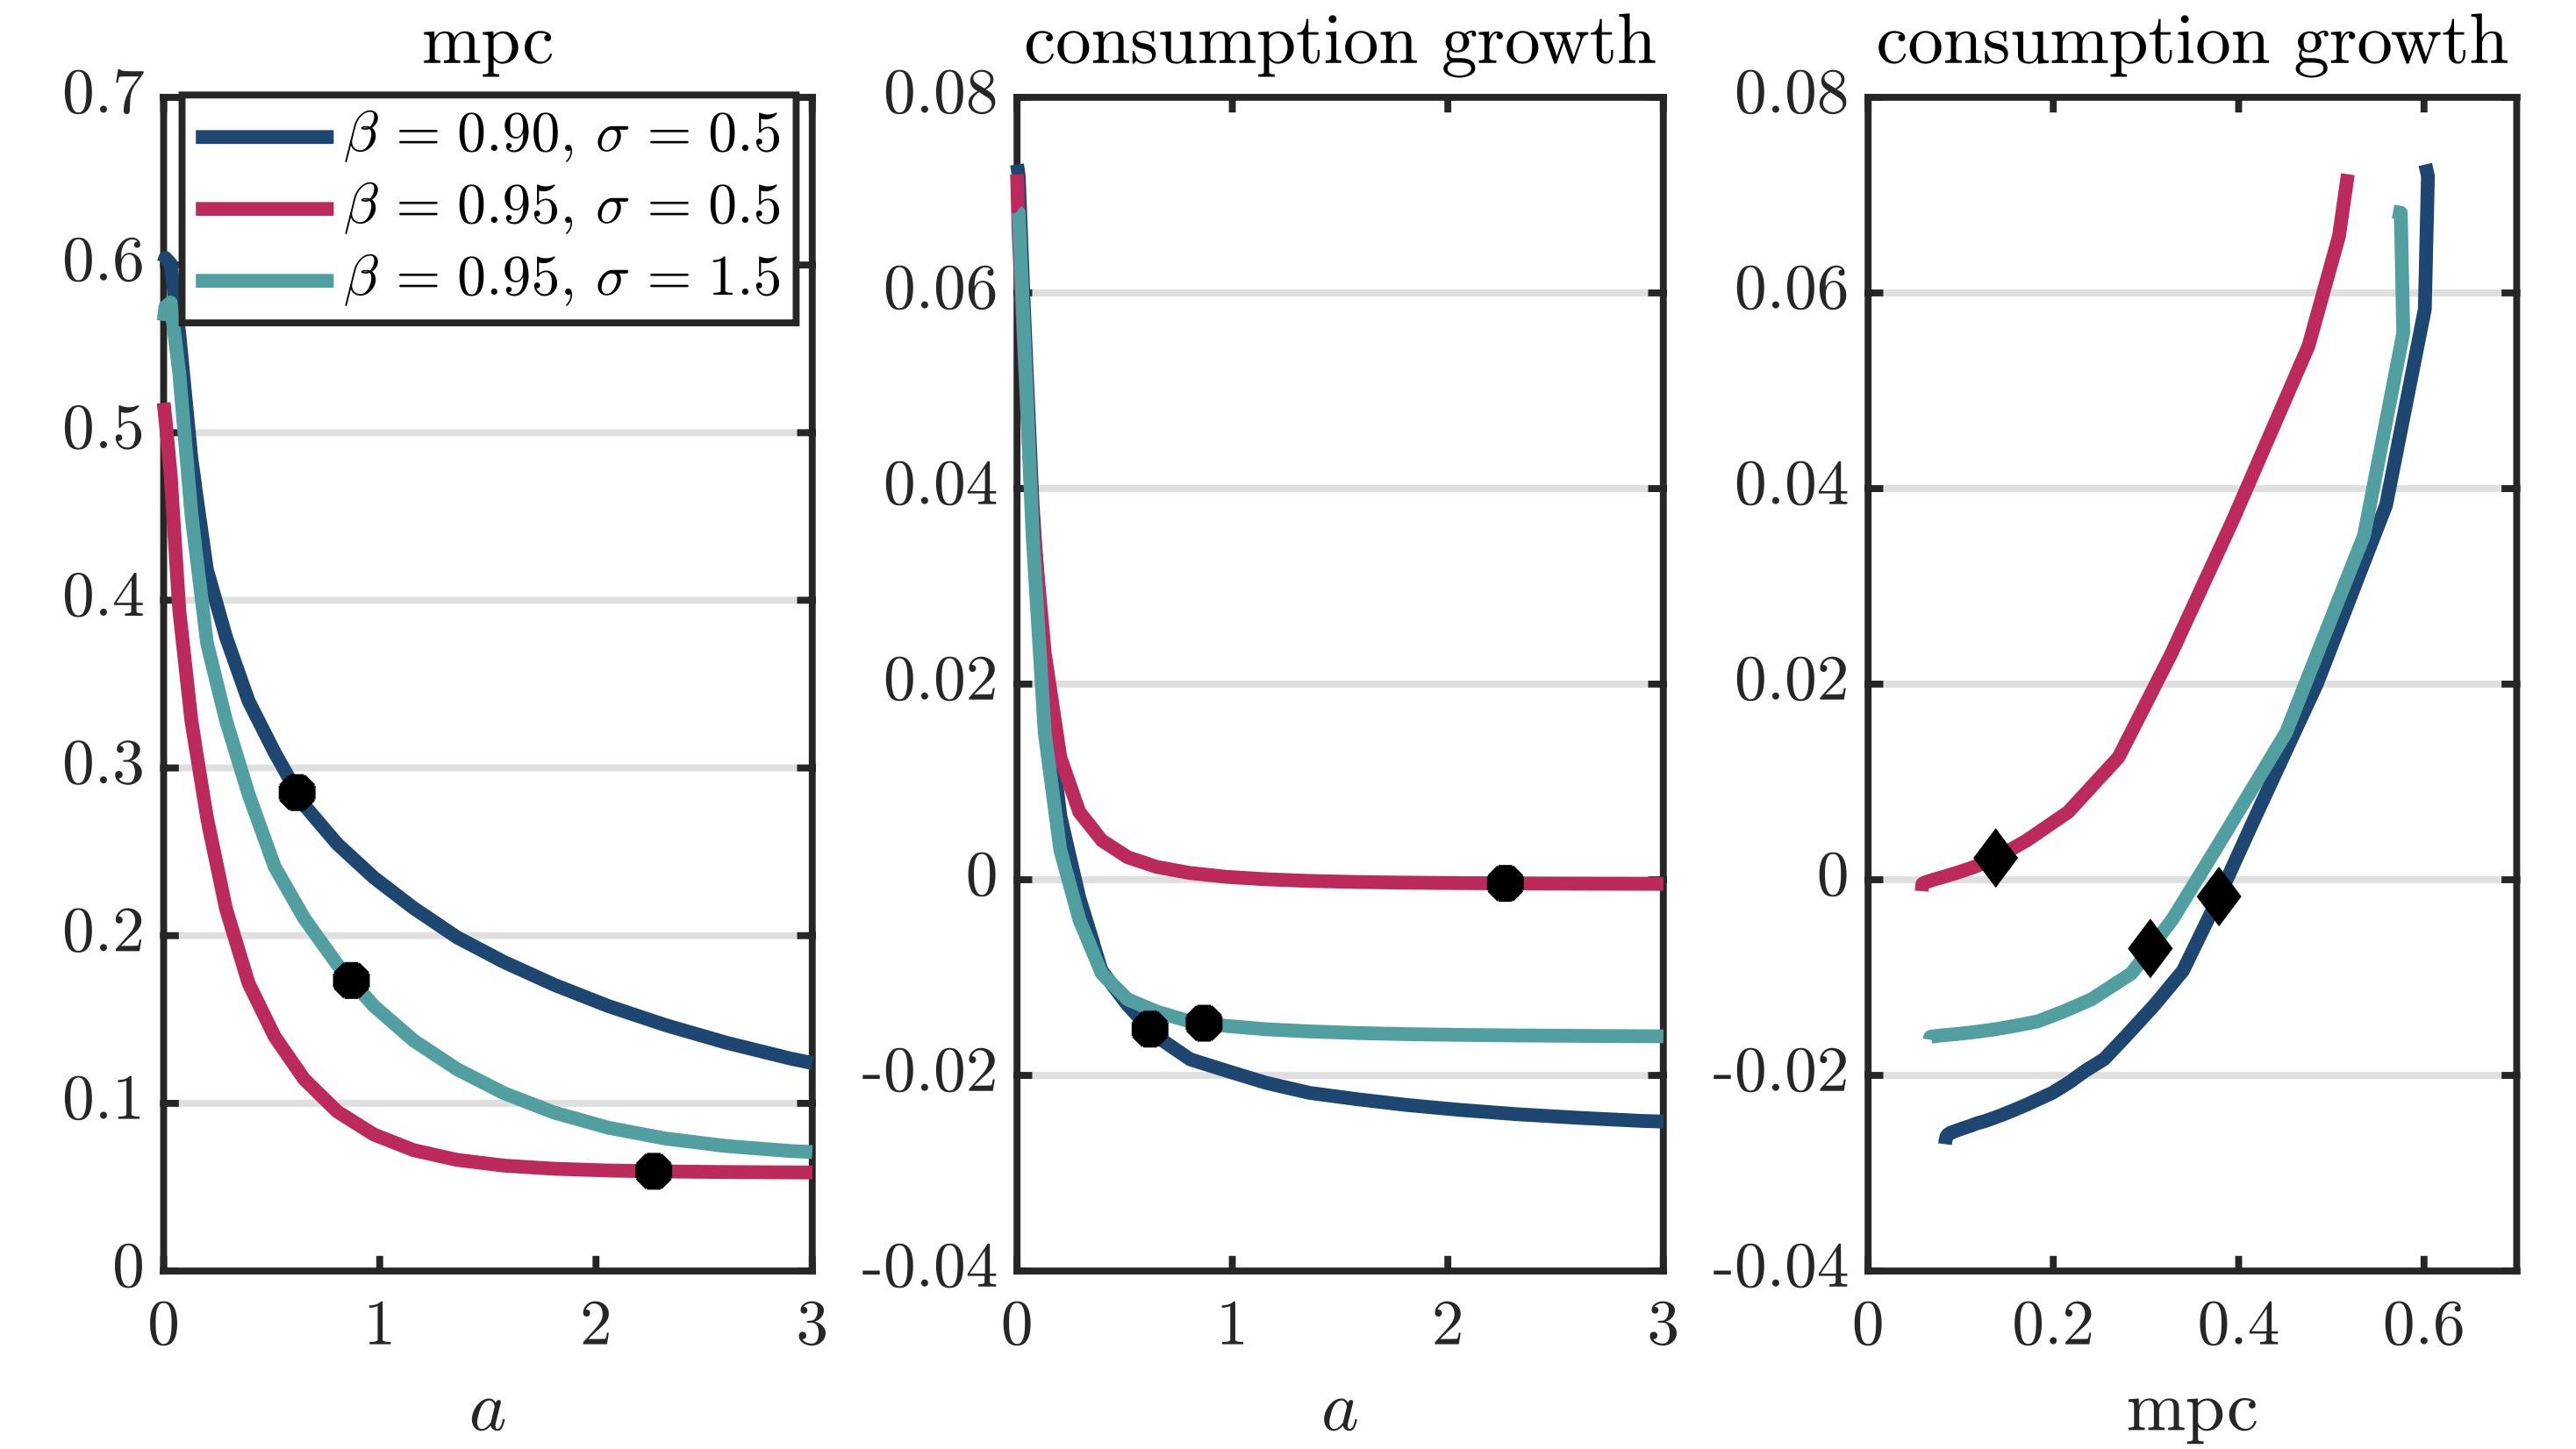
\includegraphics[width=0.7\linewidth]{Figures/baseline_model.png}
	\end{figure}

\hyperlink{fact2}{\beamerbutton{Fact 2}}
\end{frame}
\begin{frame}{Identifying the H2M}
	\begin{itemize}
		\item <1-> Two type of H2M:
		\begin{itemize}
			\item<2-> \textit{\textbf{$H2M_{NW}$}}: \footnotesize{HHs with net worth less than two months of income. (based on \cite{zeldes1989consumption})}
			\item<3-> \textit{\textbf{$H2M_{LIQ}$}}: \footnotesize{HHs with negative liquid wealth with absolute value greater than 16.5\% of annual earnings,13 or non-negative, but small, liquid wealth equal to a week or less of earnings. (based on \cite{kaplan2014model})}
		\end{itemize}
		\item<4->[]\begin{figure}
			\centering
			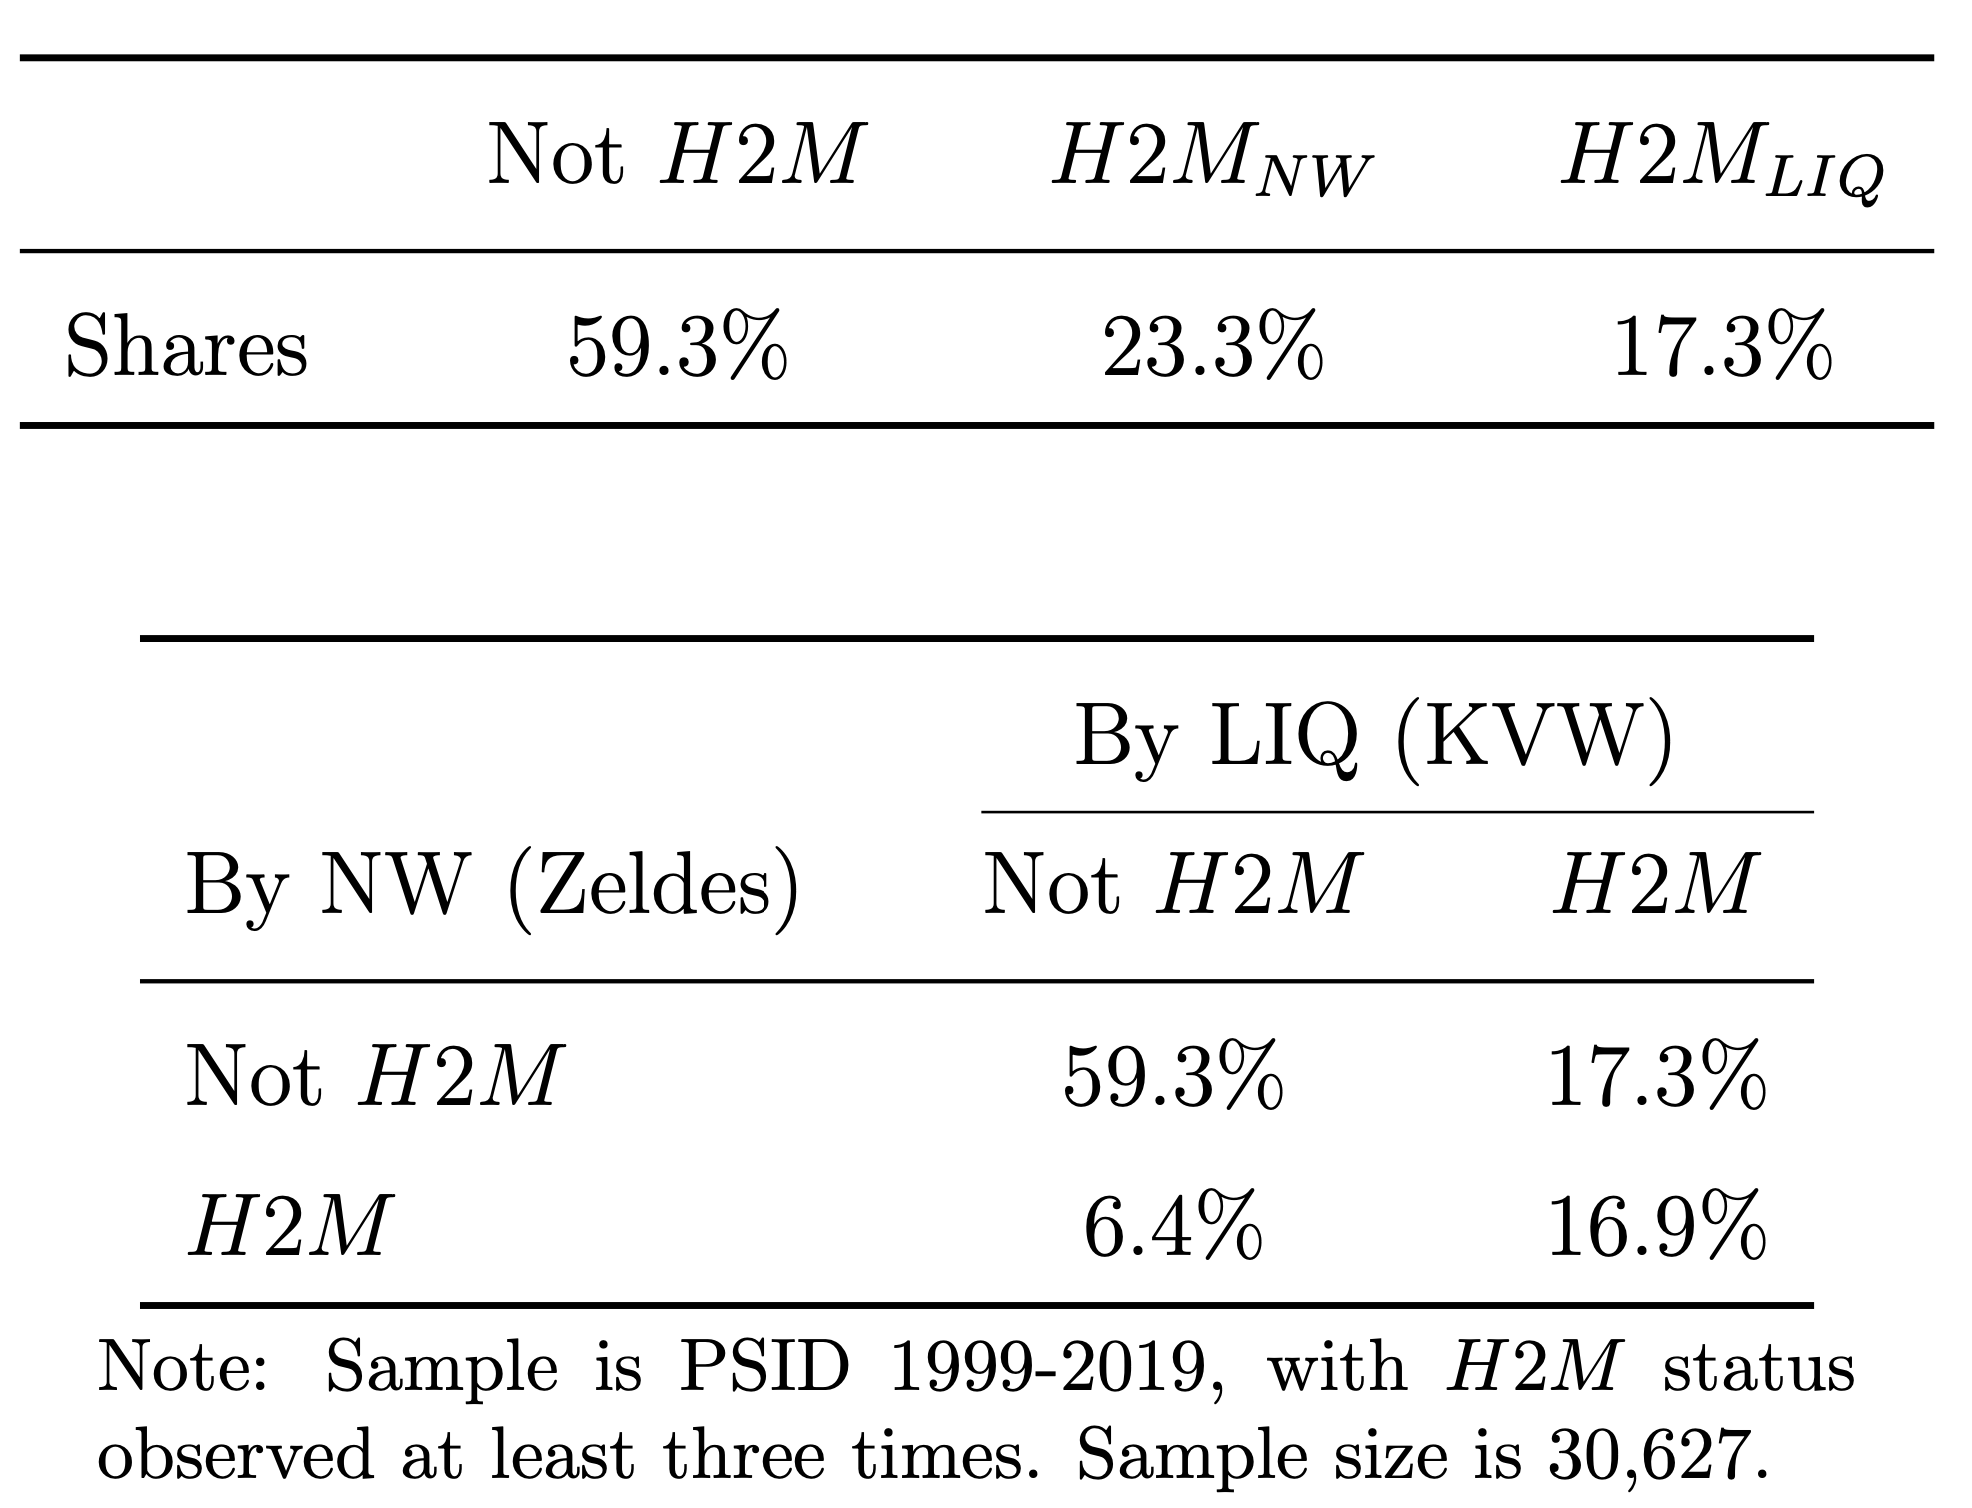
\includegraphics[width=0.5\linewidth]{Figures/Tabel1.png}
		\end{figure}
	\end{itemize}
\end{frame}
\begin{frame}{Characteristics of H2M}
	\begin{figure}
		\centering
		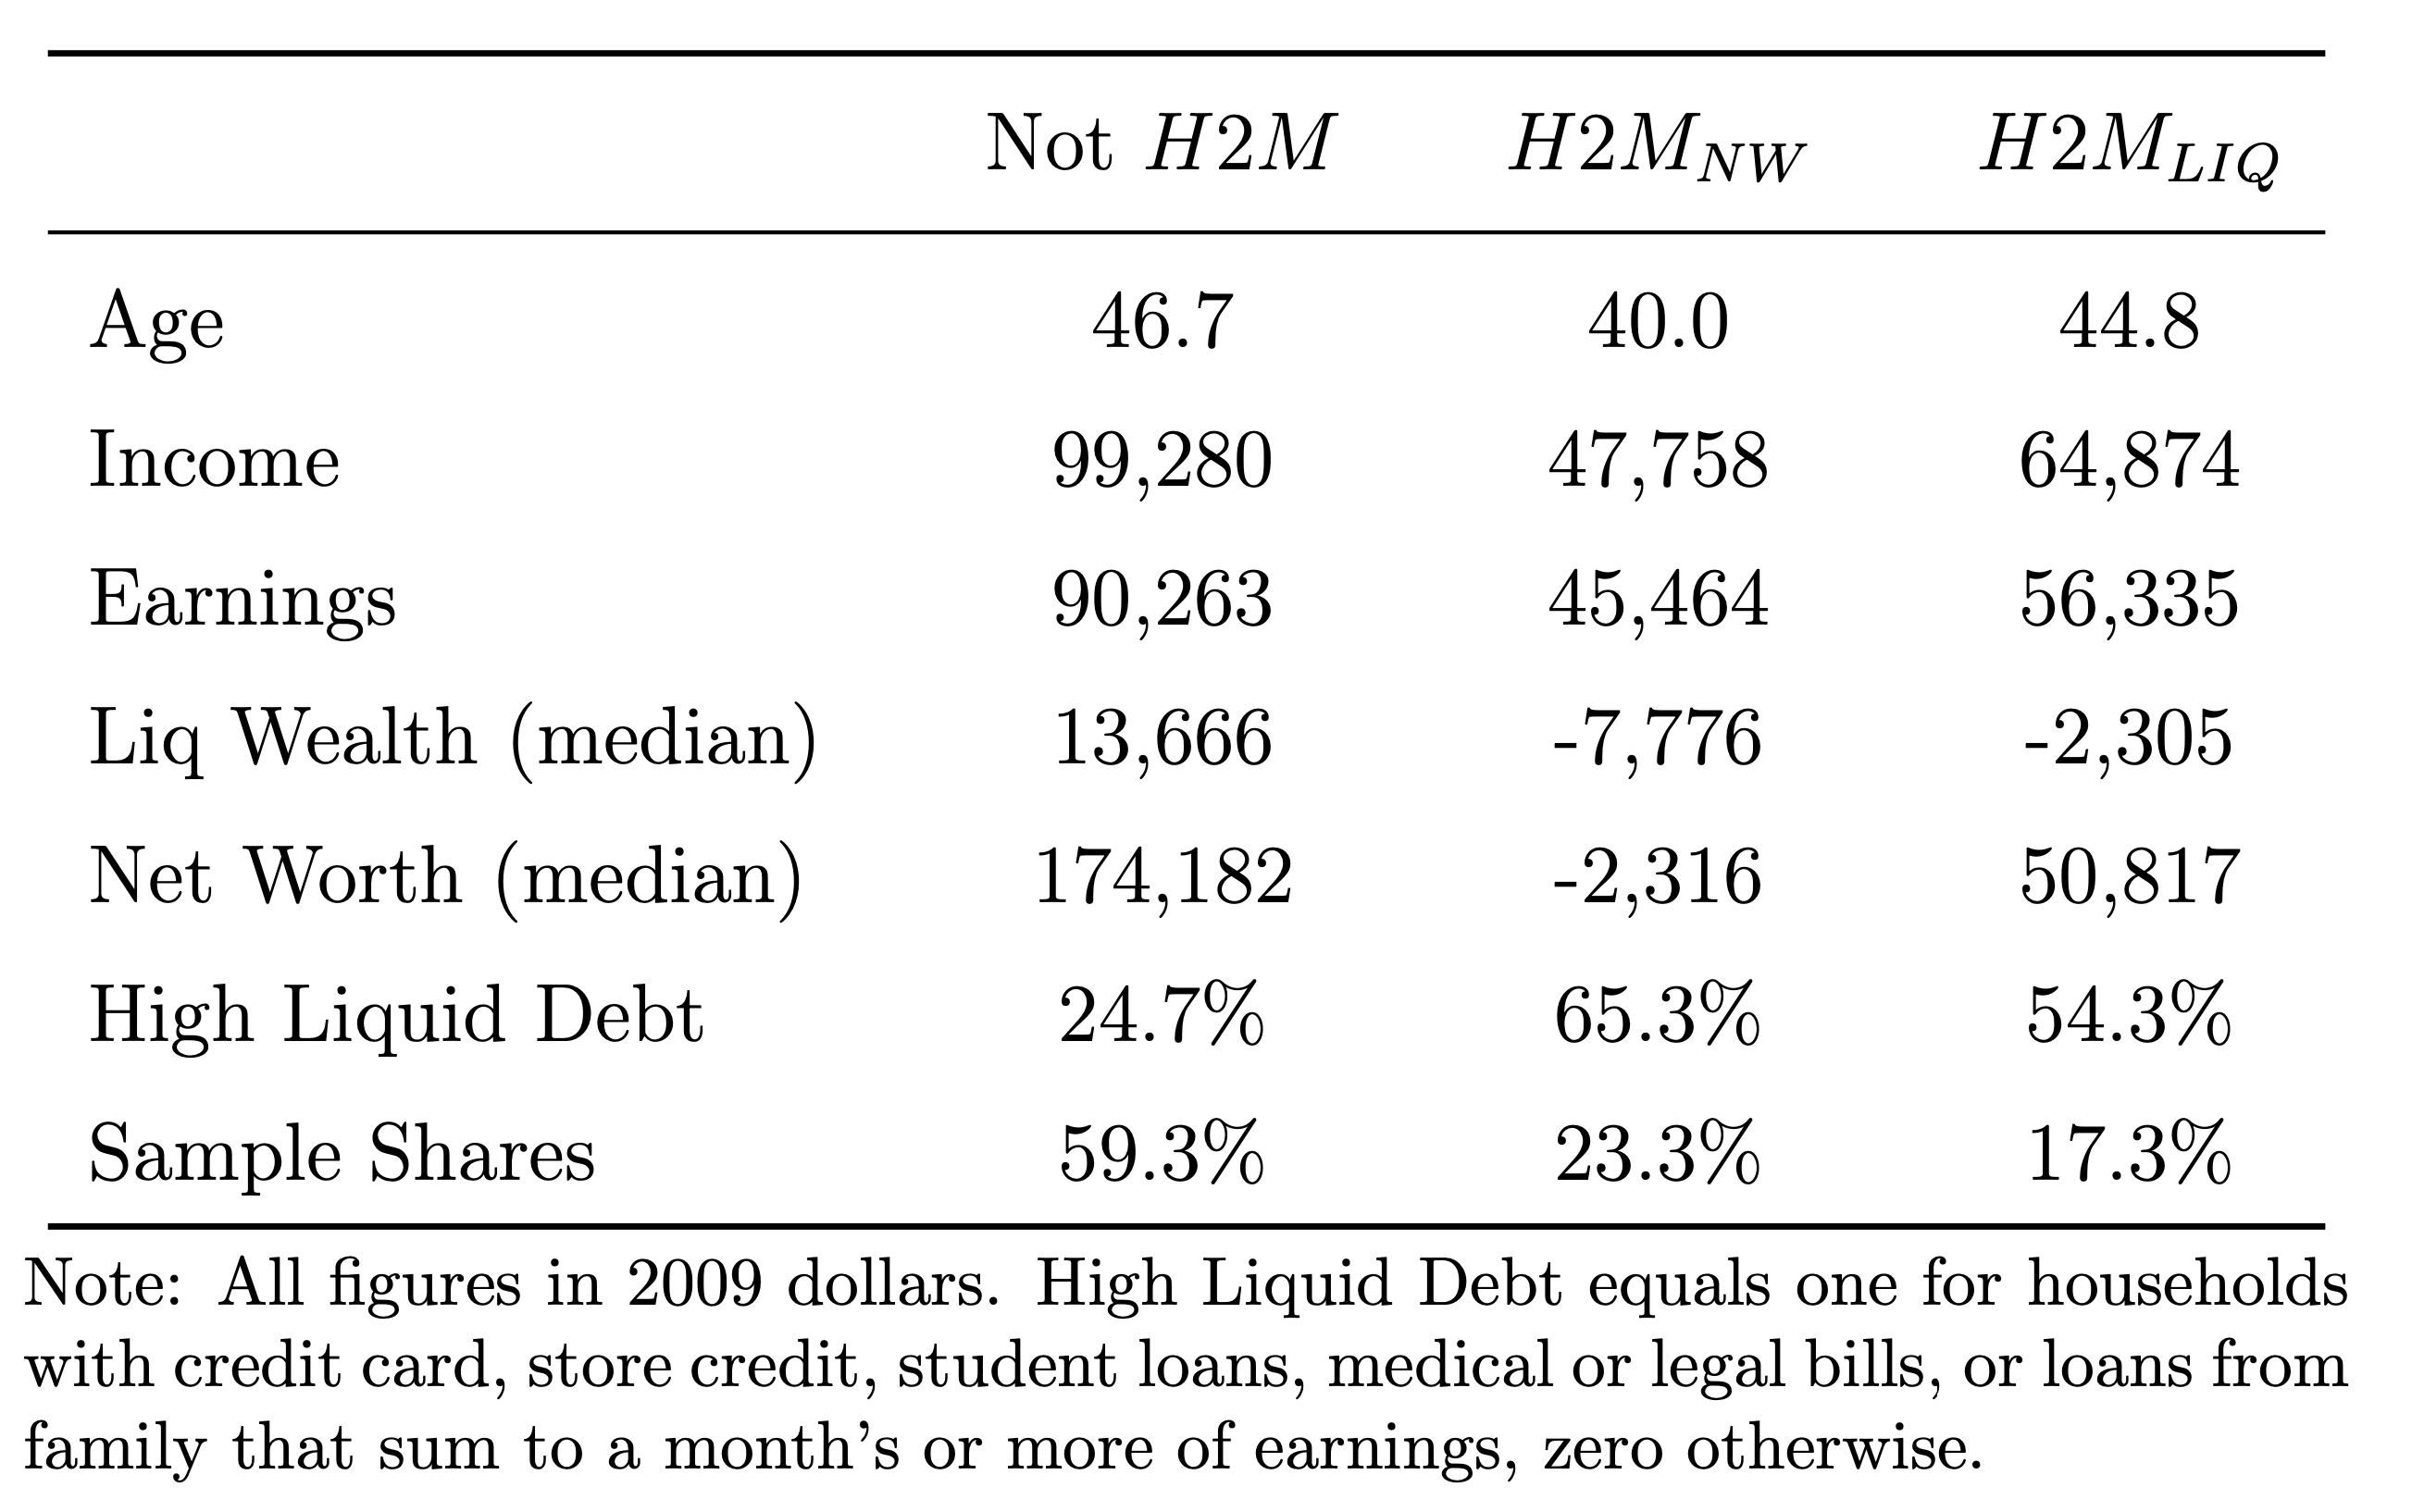
\includegraphics[width=0.7\linewidth]{Figures/Table2.png}
	\end{figure}
\end{frame}

\begin{frame}{Fact 1 - 
	Households Tend to Remain H2M}
	\begin{figure}
		\centering
		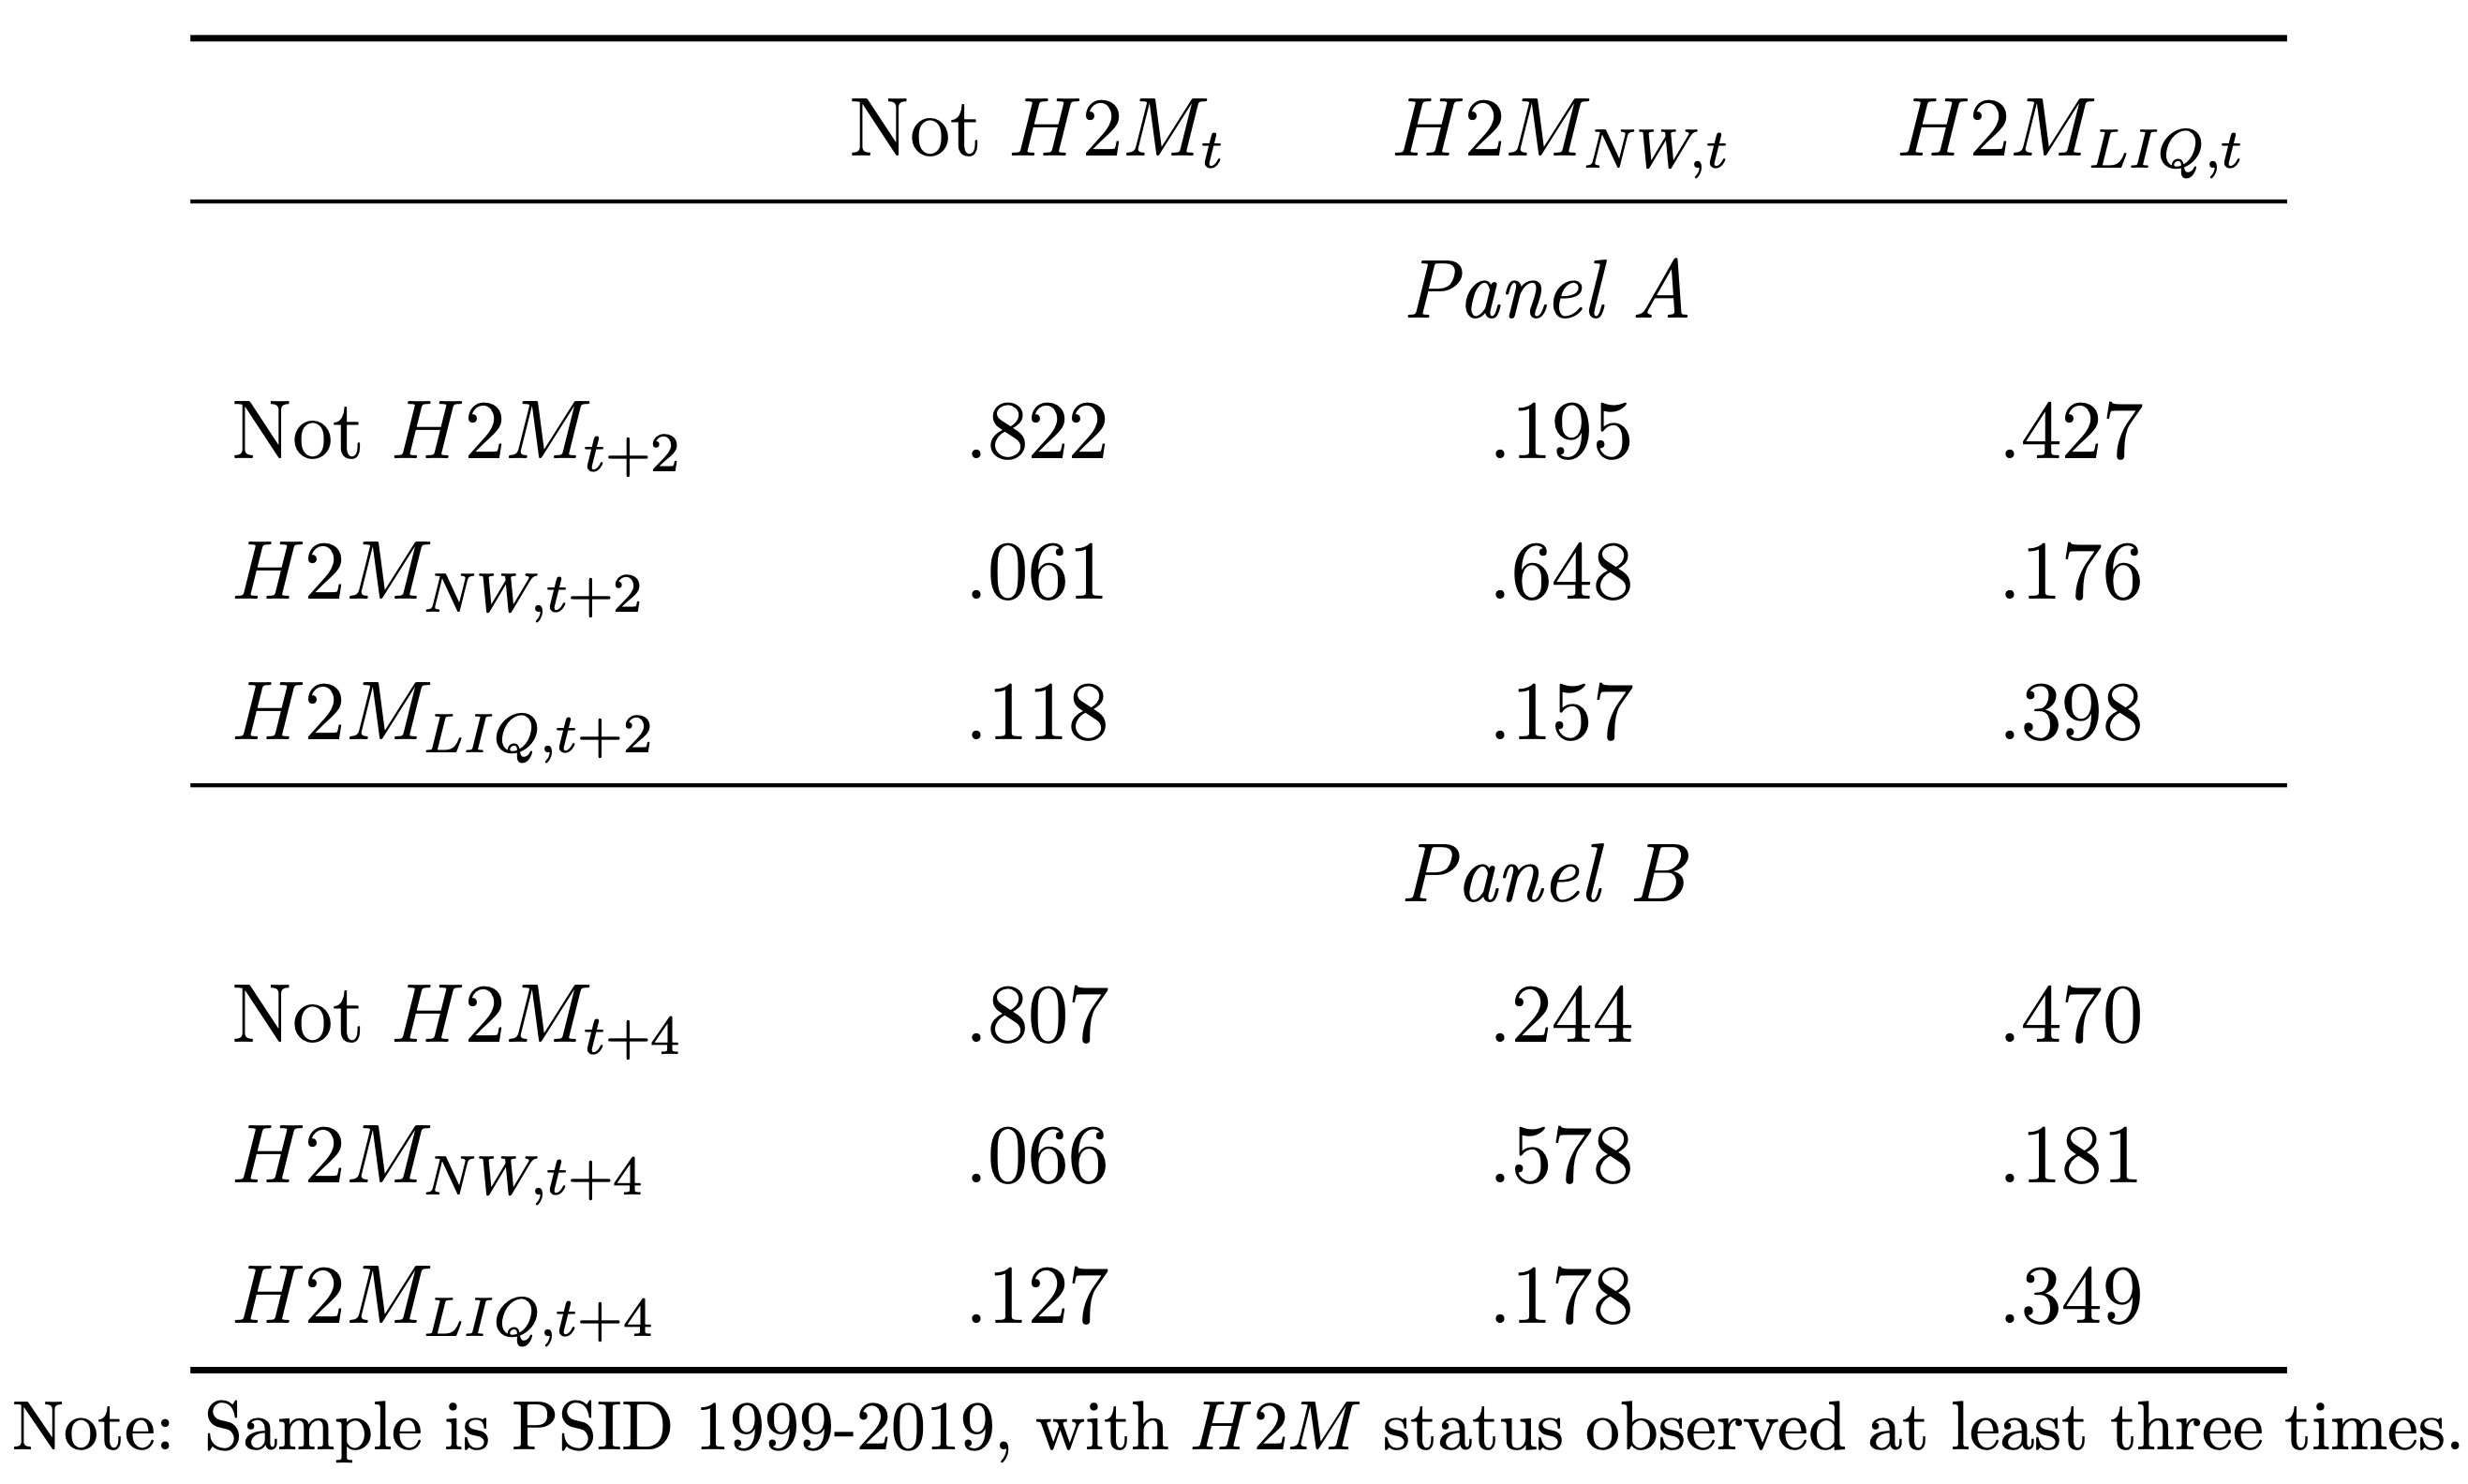
\includegraphics[width=0.7\linewidth]{Figures/Table3.png}
	\end{figure}
\end{frame}

\begin{frame}{Fact 2 - 
	H2M Do Not Have Higher Consumption Growth}
	\label{fact2}
	\begin{figure}
		\centering
		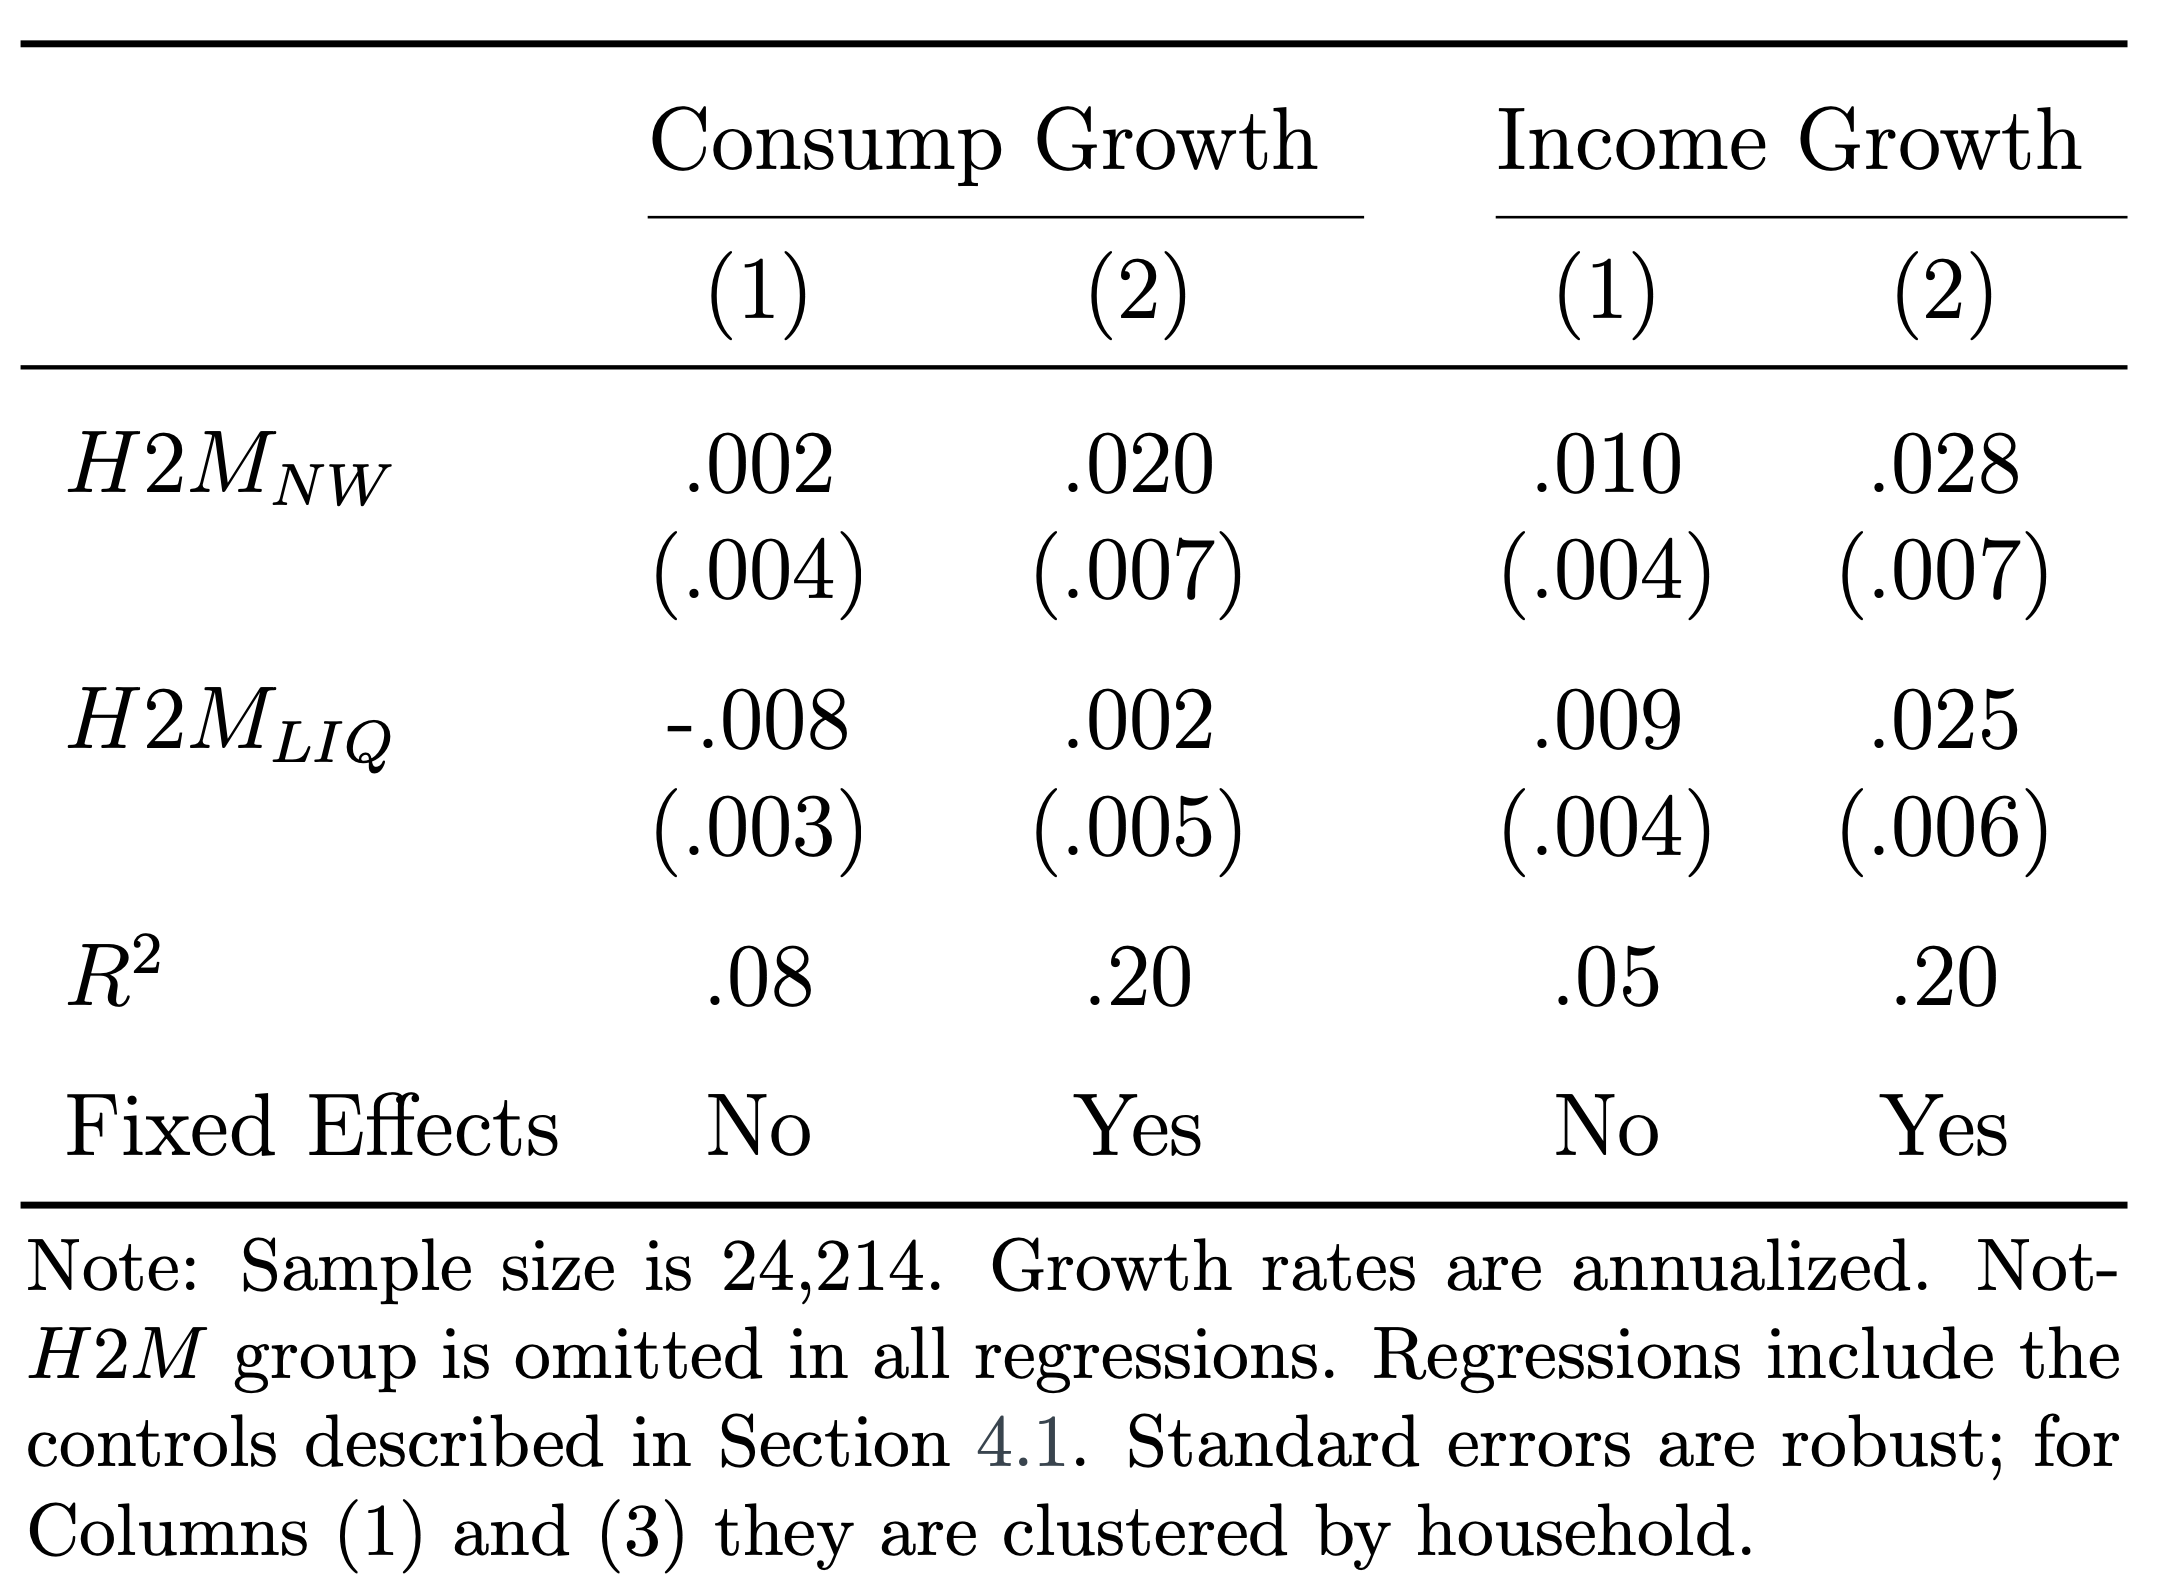
\includegraphics[width=0.7\linewidth]{Figures/Table4.png}
	\end{figure}

\hyperlink{canonical}{\beamerbutton{Canonical Model}}
\end{frame}
\begin{frame}{Fact 3 - H2M Have More Volatile Consumption and Income}
	\label{fact3}
	\begin{figure}
		\centering
		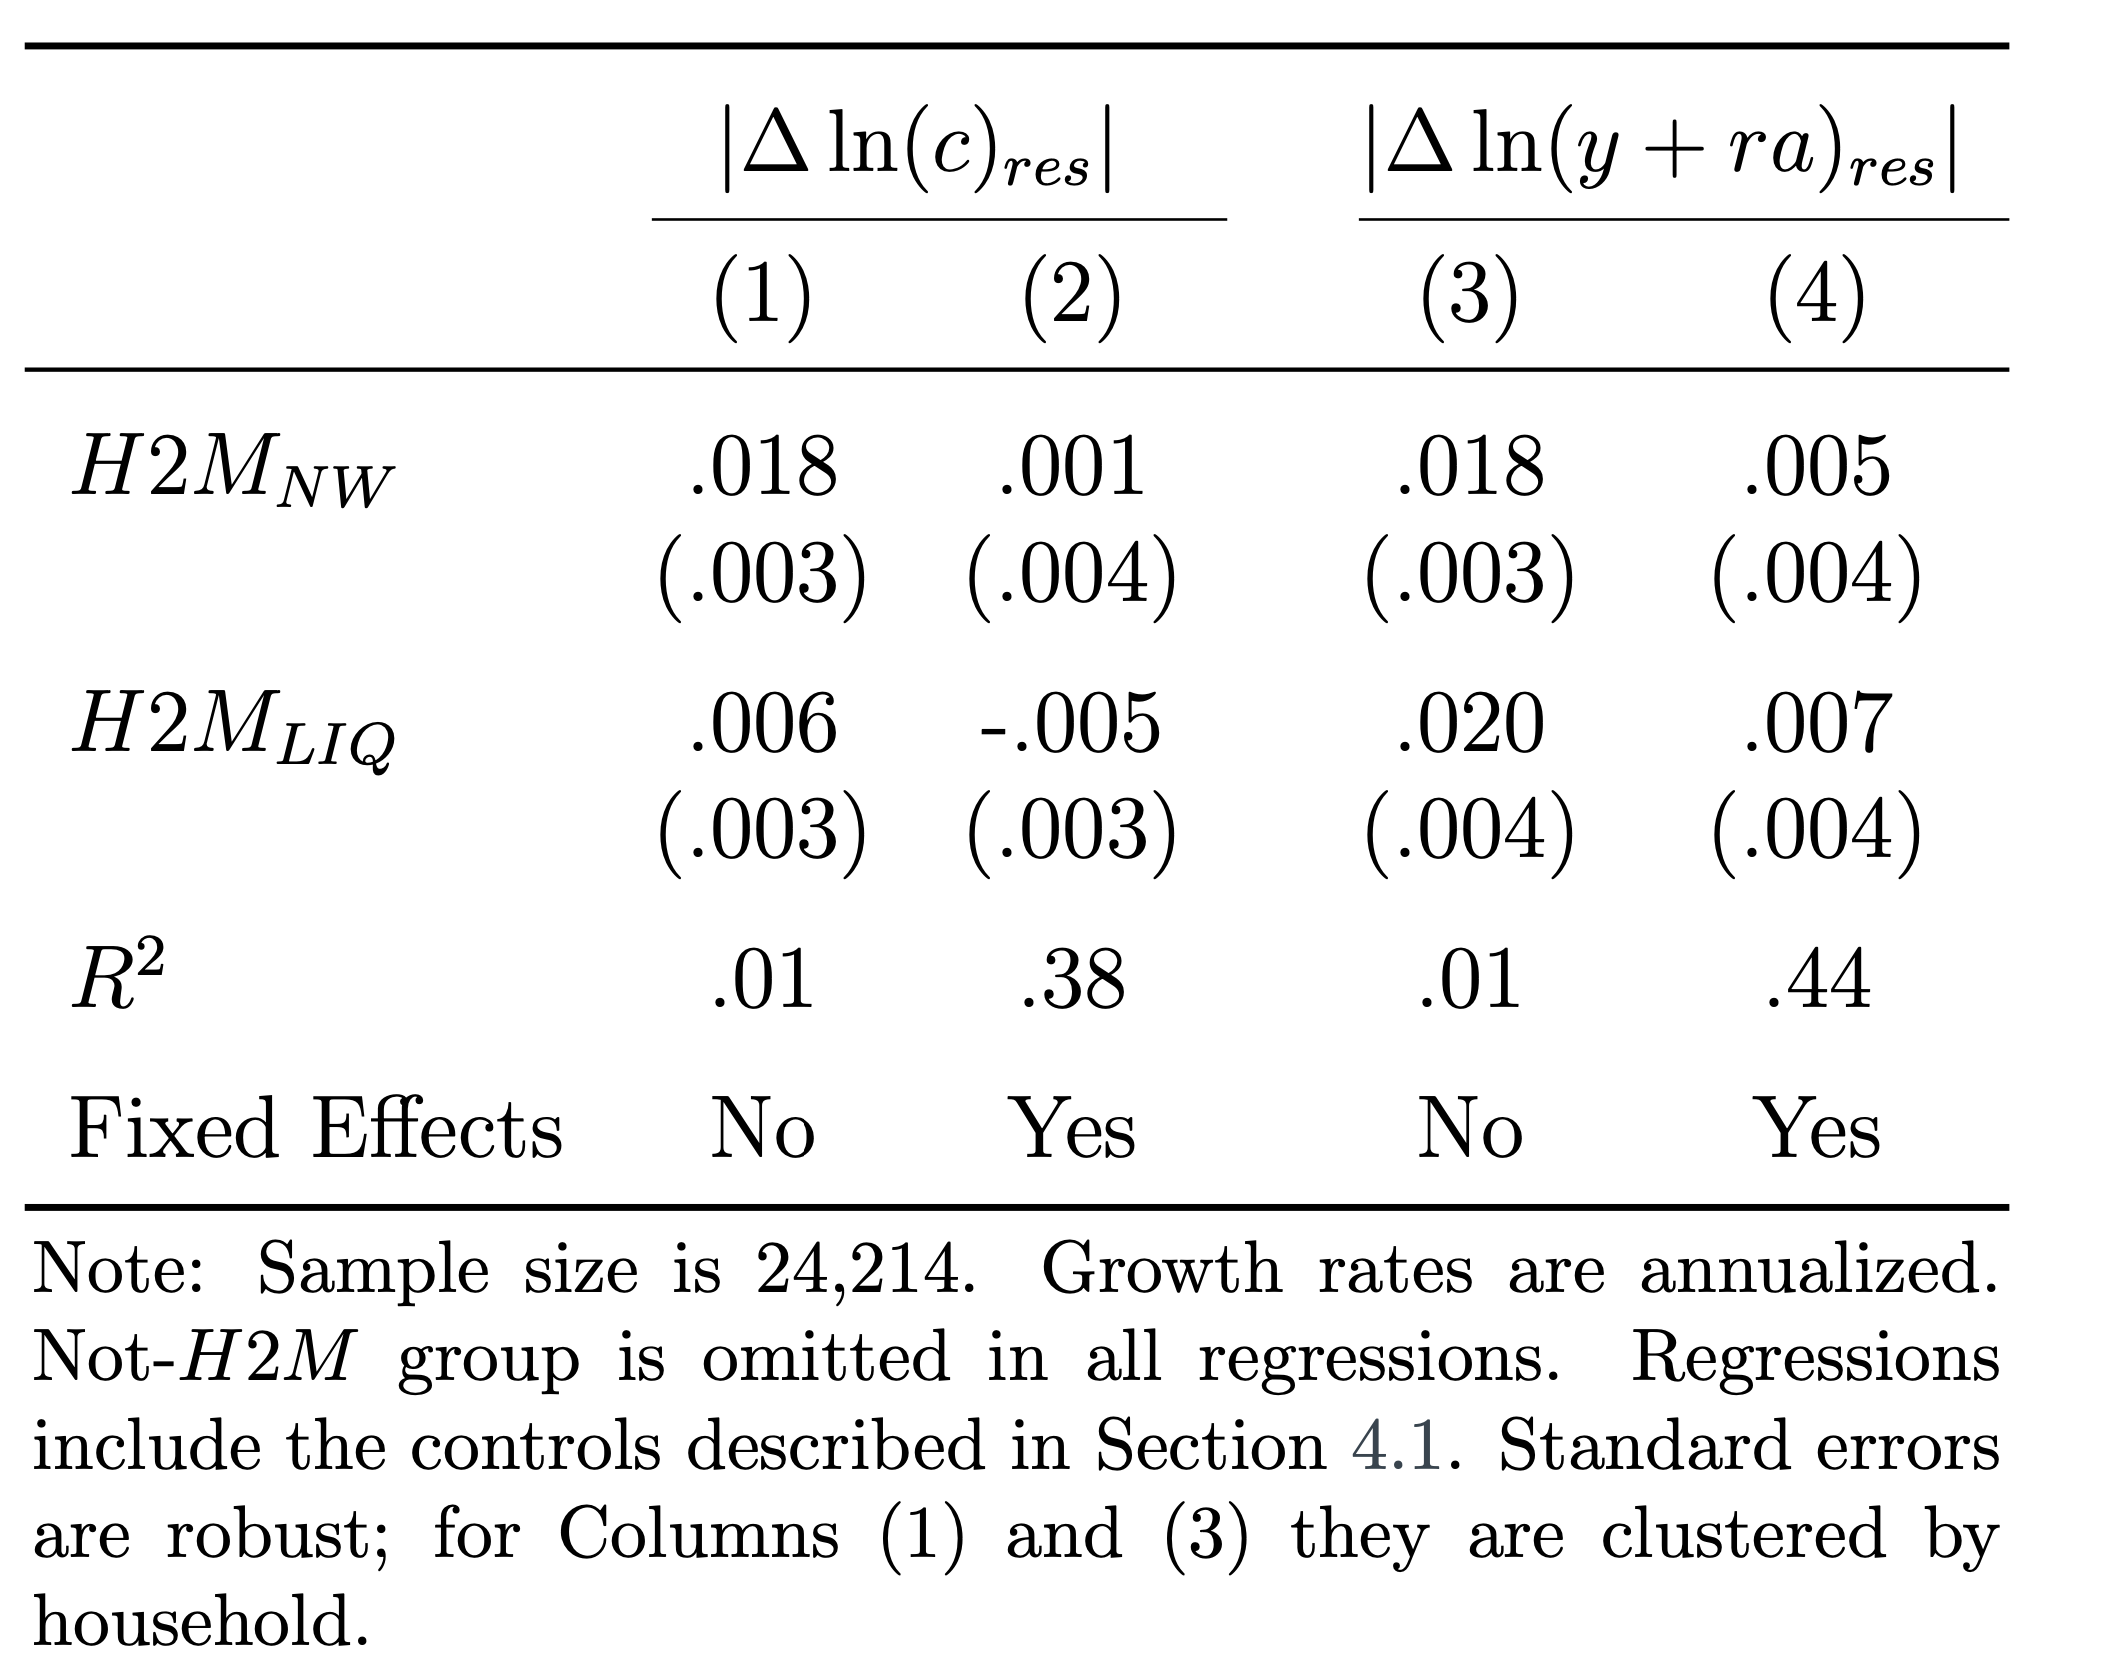
\includegraphics[width=0.7\linewidth]{Figures/Table5.png}
	\end{figure}
\end{frame}

\begin{frame}{Fact 4 - H2M Are More Elastic at Extensive Spending Margin}
	\label{fact4}
	\begin{figure}
		\centering
		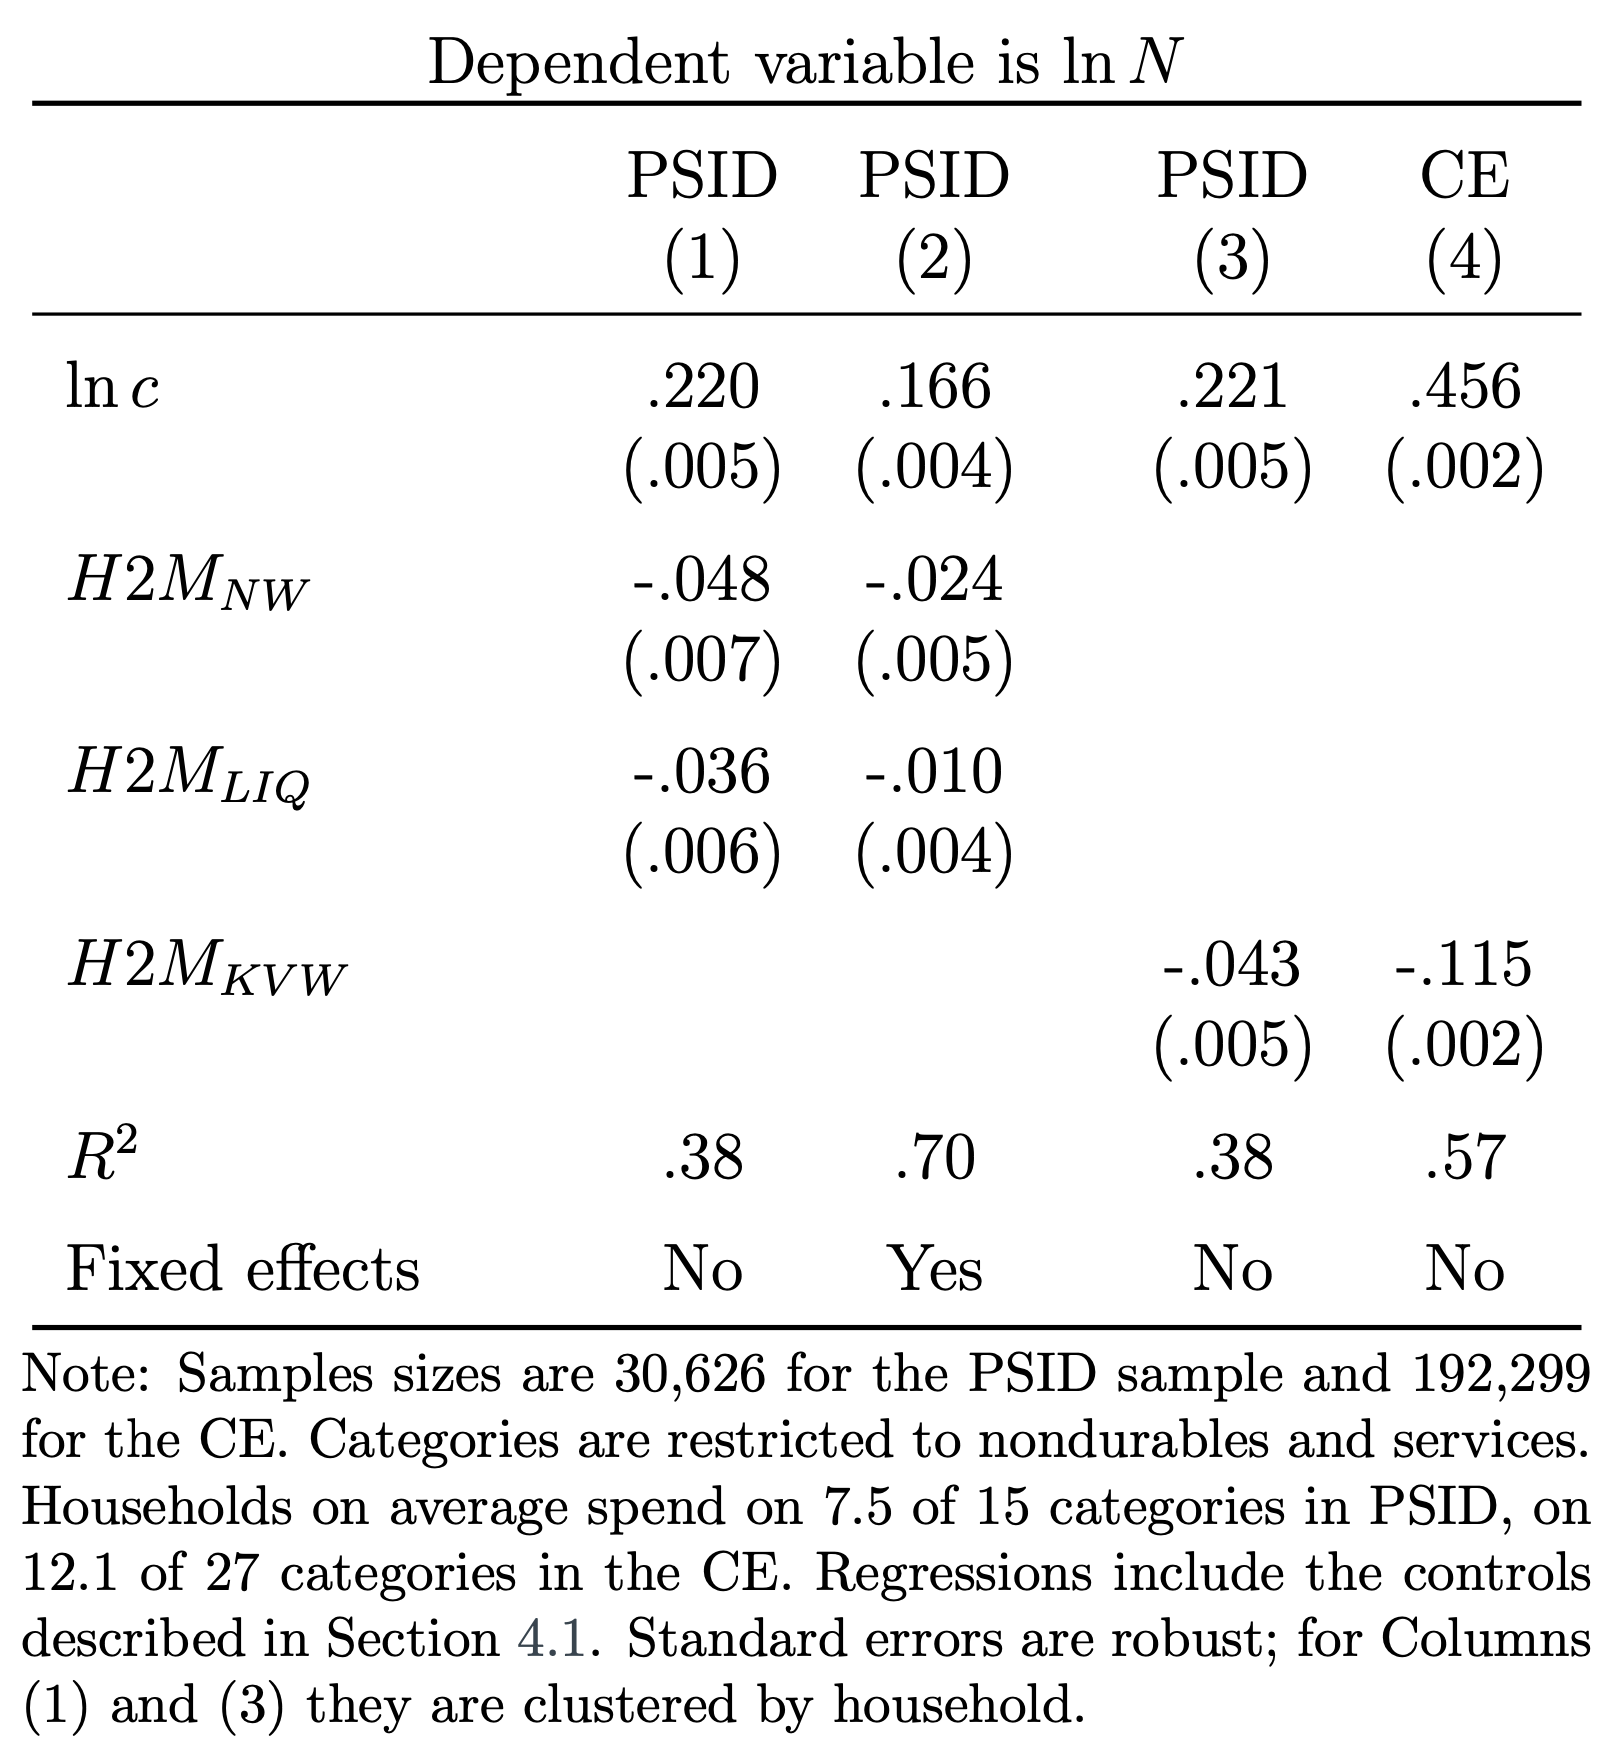
\includegraphics[width=0.5\linewidth]{Figures/Table6.png}
	\end{figure}
\end{frame}

\begin{frame}{Model Setup}
	The mentioned facts show that preference heterogeneity plays a key role in the H2M behavior.
	\begin{itemize}
		\item <1-> They calibrate the model with 3 different type of HHs:
		\begin{figure}
			\centering
			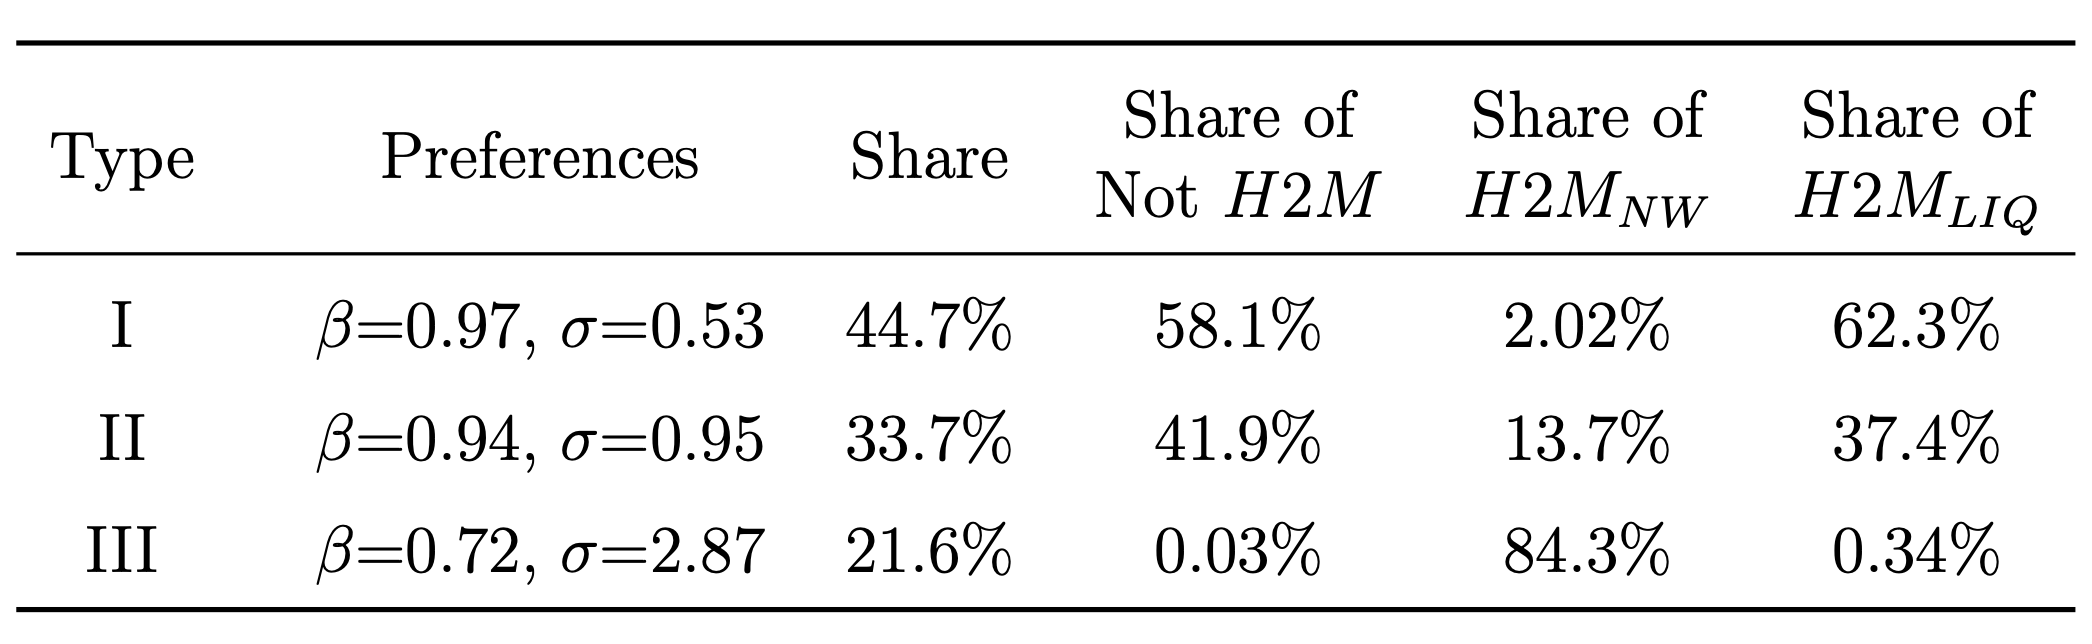
\includegraphics[width=0.7\linewidth]{Figures/Table10.png}
		\end{figure}
	\end{itemize}
\end{frame}
\begin{frame}{Results}{Calibration Results}
	\label{table13}
	\begin{figure}
		\centering
		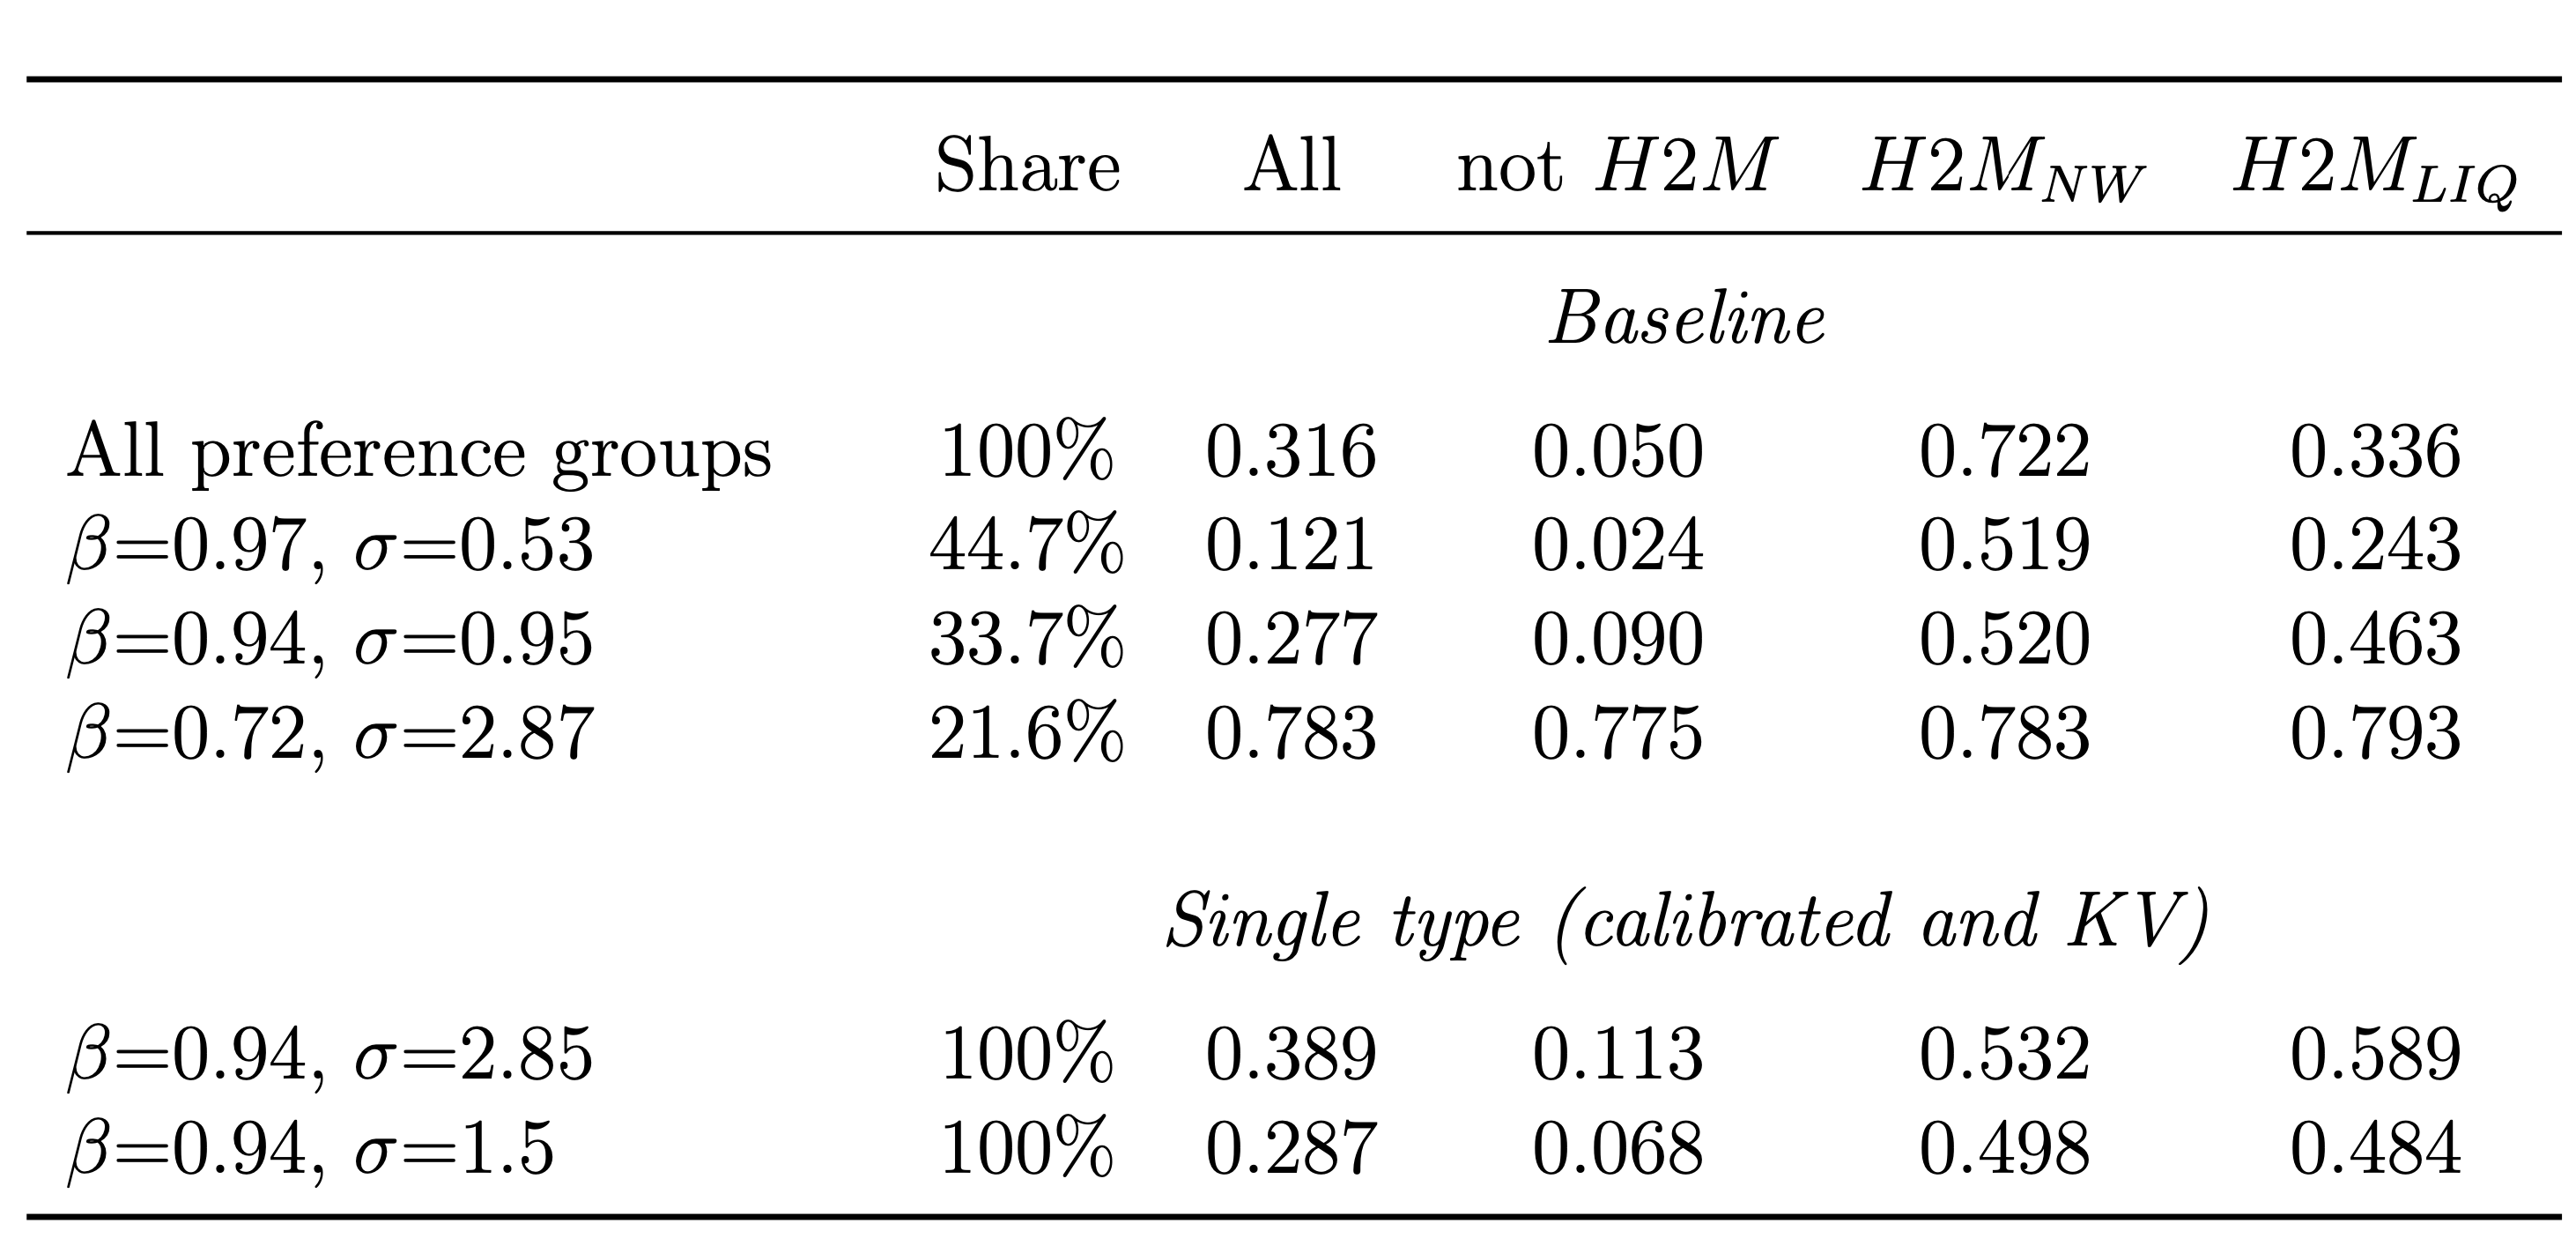
\includegraphics[width=0.85\linewidth]{Figures/Table13.png}
	\end{figure}
\end{frame}



\scriptsize 
	\begin{frame}[allowframebreaks]{References}
			\bibliographystyle{aea}
\bibliography{ref.bib}
		
	\end{frame}
	
	\normalsize
\end{document}
